%!TEX root = ../report.tex

\section{Schnelligkeit}
Schnelligkeit ist die Fähigkeit in ermüdungsfreiem Zustand mit möglichst kurzen zeitlichem Abstand auf einen Reiz zu reagieren oder zu agieren.
\begin{figure}[H]
  \centering
  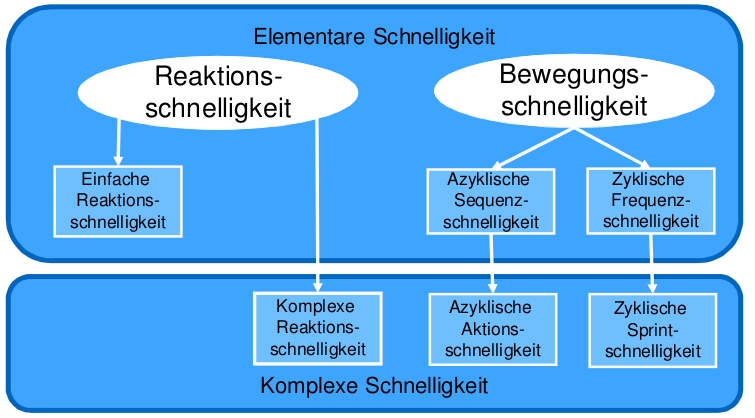
\includegraphics[width=.5\textwidth]{pictures/schnelligkeit_overview.png}
  \caption{Überblick Schnelligkeit}
\end{figure}
\begin{figure}[H]
  \centering
  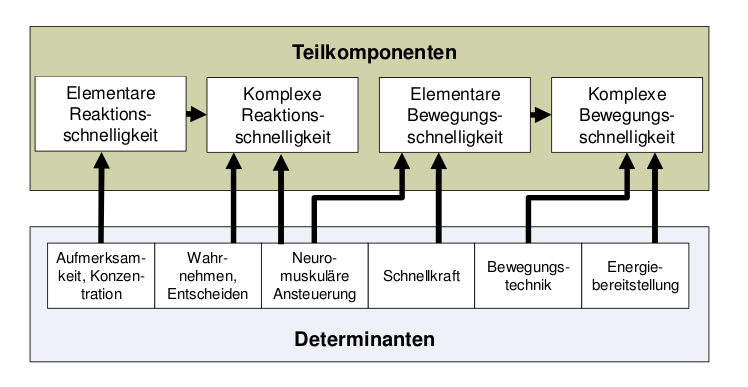
\includegraphics[width=.5\linewidth]{pictures/schnelligkeit_determinanten.png}
  \caption{Determinanten der Schnelligkeit}
\end{figure}

\subsection{Begriffe, Systematik und Determinaten}
\subsubsection{Reaktionsschnelligkeit}
\begin{description}
  \item[Reaktionsfähigkeit] ist die psychophysische Fähigkeit auf Reize schnell zu reagieren.
  \item[Elementare Reaktionsschnelligkeit] Kleinmotorische Bewegungsantworten auf einfache Reize
  \item[Komplexe Reaktionsschnelligkeit] Großmotorische Bewegungsantworten \& komplexe (Wahl-) Reaktionen.
\end{description}

\textbf{Modell der Reaktionsgeschwindigkeit}\\
\begin{figure}[H]
  \centering
  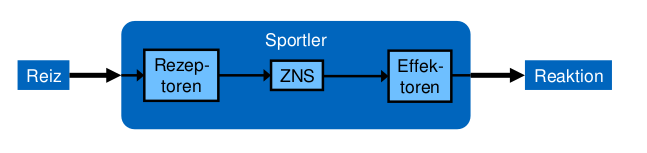
\includegraphics[width=.5\textwidth]{pictures/reaktionsgeschwindigkeit_modell.png}
  \caption{Modell der Reaktionsgeschwindigkeit}
\end{figure}
\begin{description}
    \item[Übertragung bis Rezeptor] hängt vorwiegend von den Eigenschaften des Rezeptors ab (1-20ms).
    \item[Restliche ÜBertragung] wird von den Eigenschaften des Nervensystems beeinflusst (Rezeptor $\rightarrow$ ZNS: 1-100ms, ZNS $\rightarrow$ Effektor: 10-20ms).
    \item[Verarbeitung im ZNS] wird beeinflusst von psychischen Eigenschaften wie Aufmerksamkeit und Wahrnehmung und kann von 70 bis 300ms dauern.
    \item[Verarbeitung in den Effektoren] Abhängig von neuromuskulären Eigenschaften wie Fastetypzusammensetzung oder inter-/intramuskuläre Koordination
\end{description}
Die gesammte Übertragungszeit beträgt in etwa 112 - 510ms.

\subsubsection{Bewegungsschnelligkeit}
Bewegungsschnelligkeit ist die Fähigkeit, Bewegungen in höchster Geschwindigkeit oder kürzester Zeit auszuführen.
\begin{figure}[H]
    \centering
    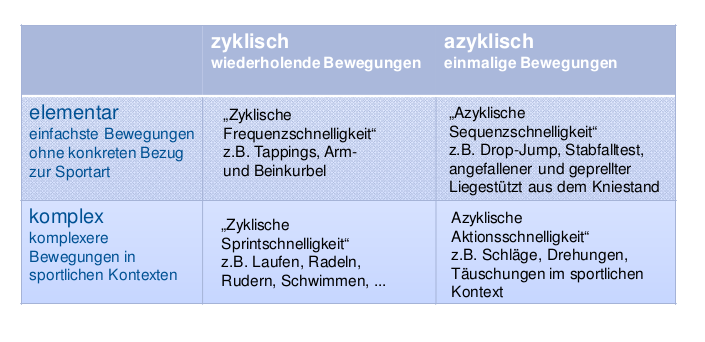
\includegraphics[width=.7\textwidth]{pictures/bewegungsgeschwindigkeit_struktur.png}
    \caption{Struktur der Bewegungsschnelligkeit}
\end{figure}

Die Bewegungsschnelligkeit hängt von drei Bereichen ab:
\begin{description}
    \item[Neuromuskuläres System] Neuronale Steuer- \& Regelprozesse, Reaktionsgeschwindigkeit, inter/intra-muskuläre Koordination,\ldots
    \item[Psychisches System] Konzentration, Wahrnehmung, Motivation, \ldots
    \item[Tendomuskuläres System] Querschnittsfläche FT-Fasern, Stiffness, Viskosität, \ldots
\end{description}

\subsection{Trainingsmethoden}
Schnelligkeit ist schlechter zu trainieren als Ausdauer oder Kraft.\\
Zu trainierende Determinanten sind:
\begin{figure}[H]
    \centering
    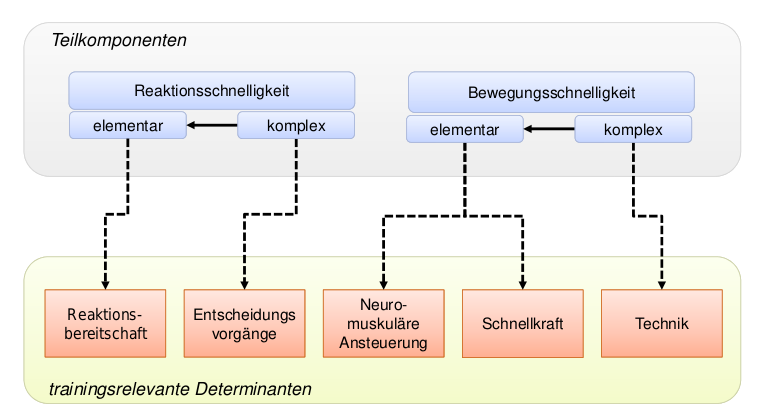
\includegraphics[width=.7\textwidth]{pictures/schnelligkeit_trainierbare_determinanten.png}
    \caption{Trainierbare Determinanten}
\end{figure}

\paragraph{Belastungsnormative}
\begin{description}
    \item[Intensität] Bewegung auf maximaler Geschwindigkeit
    \item[Dauer] 8-10s, Abbruch bei Erschöpfung
    \item[Pause] bis vollständig regeneriert, Schnelligkeitstraining vor anderen
    \item[Durchführung] Mit maximaler Konzentration \& Willen, mit Aufwärmen
\end{description}

\subsubsection{Reaktionsbereitschaft}
Training beinhaltet einfache Reaktionen (Pfiff, (Nacken- :P) Klatschen) auf akustische, visuelle oder taktile Reize.

\subsubsection{Entscheidungsvorgänge}
Eine Wahlreaktion wird vor einer motorischen Reaktion eingefordert.
Auch die richtige Wahrnehmung ist wichtig, Signal wird erschwert zu verstehen (leiser Pfiff = noop, lauter Pfiff = go)

\subsubsection{Neuromuskuläre Ansteuerung}
Grundbewegungen schnell realisieren. Es wird unterschieden zwischen zyklischen (wiederholenden) und azyklischen (einmaligen) Bewegungen.
\paragraph{Geschwindigkeitsbarriere} Häufige Realisation der Maximalgeschwindigkeit führt zu einer Verfestigung der neuromuskulären Ansteuerung (Reizleitungswege, Innervationsmuster).
Gegenmaßnahmen sind nur wenig Wettkampfsimulationen mit Maximalgeschwindigkeit (1/Woche), Variation der Bewegung und Entwicklung der elementaren Fähigkeiten
\paragraph{Erleichterte Bedingungen} Erleichtern der Übungen durch verringern des Wiederstands oder Körpergewichts um Geschwindigkeit zu erhöhen.
Beispiele sind Treppenläufe bergab (zyklisch) oder leichtere Wurfgeräte (azyklisch).
\paragraph{Räumliche Zwänge} Erzwingen einer höheren Frequenz durch Einengungen (z.B. Fesseln).
\paragraph{Mentales Training} Der Carpenter-Effekt (Denken an eine Bewegung bewirkt diese in einem abgeschwächtem Maß) wird dazu genutzt mit Metaphern in der Übungsbeschreibung eine Aktion hervorzurufen (``Springe wie ein Frosch'').
\paragraph{Elektromyostimulation} Elektrische Stimulation auf das Innervationsmuster. Die nicht belegte Hypothese ist dass dadurch eine bessere Rekrutierung motorischer Einheiten erfolgt und das bestehende Innervationsmuster ``überschrieben'' wird.

\subsection{Technik}
Technikübungen sind disziplinspezifisch, schnell ausgeführte Bewegungen die meist überbetont werden.
Kombinationen aus einzelnen Aktionen und Übungen sind möglich.
